\chapter{Strahlenoptik}

In diesem Kapitel charakteriesiert der Begriff „geometrische Merkmale“ die konzeptuellen Merkmale des abstrakten Models eines optischen Gerät,
und der Begriff „gestalterische Merkmale“ die Merkmale der Darstellung des Gerät auf einer Zeichenebene.

\section{Ebene Spiegel}

Die geometrische Merkmale eines ebenen Spiegel ist die Ebene, auf die ein Lichtstrahl trifft.
Diese Ebene wird durch einen Normalvektor und einen zentralen Punkt charakterisiert.

\begin{asycode}
vector normalDir = (0, 1);
point centerM = (0, 0);
PlanaMirror m = PlanaMirror(normalDir, centerM);
\end{asycode}

Möchte man den Spielgel auf einer Zeichenebene bringen, muss man gestalterische Merkmale feststellen.
Sie sind die Abstände vom zentralen Punkt in Richtungen Link und Rechts, sowie die Stärke.

\begin{asycode}
m.setupMirrorSize(leftWidth=25, rightWidth=20, mirrorThickness=1)
 .drawMirror();
\end{asycode}

Wenn die Abstände vom zentralen Punkt in beide Richtungen gleich sind, kann man die kurze Form benutzen.

\begin{asycode}
m.setupMirrorSize(leftWidth=25)
 .drawMirror();
\end{asycode}

Hier wird der Stärke mit dem Standartwert \texttt{mirrorThickness} gesetzt.
Man findet den Wert in der Datei \texttt{optik.asy}.

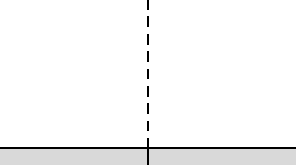
\includegraphics{asy/blankmirror.pdf}

\input{asy/blankmirror.tex}

Möchte man den Einfallstrahl und den reflektierten Strahl zeichnen, muss man den Einfallpunkt und den Einfallslot berechnen.